\documentclass[UTF8,aspectratio=169]{ctexbeamer}
\usetheme{Madrid}
\usecolortheme{default}
\usepackage{amsmath}
\usepackage{booktabs}
\usepackage{siunitx}
\usepackage{array}
\usepackage{xcolor}
\usepackage{xurl}
\usepackage{colortbl}
\usepackage{bm}
\usepackage{graphicx}

\newcommand{\good}[1]{\textcolor{green!45!black}{#1}}
\newcommand{\warn}[1]{\textcolor{red!65!black}{#1}}
\newcommand{\bluenote}[1]{\textcolor{blue!65!black}{#1}}
\newcommand{\src}[1]{\vfill{\tiny\textcolor{gray!75!black}{Source: \url{#1}}}}
\newcolumntype{L}[1]{>{\raggedright\arraybackslash}p{#1}}
\newcolumntype{R}[1]{>{\raggedleft\arraybackslash}p{#1}}
\newcolumntype{C}[1]{>{\centering\arraybackslash}p{#1}}

\definecolor{winrow}{RGB}{220,240,220}
\definecolor{softrow}{RGB}{232,242,255}
\definecolor{warnrow}{RGB}{255,235,230}

\title[Tier-3A Family-Aware Head]{Tier-3A LONO Ablation\\Family-Aware $\mu$-Head vs.\ Single-Head Baseline}
\author{Mie Spray Postprocessing Project}
\date{\today}

\begin{document}

\begin{frame}
  \titlepage
\end{frame}

% ──────────────────────────────────────────────────────────────
\begin{frame}{Message}
\small
\textbf{Claim:} replacing the single $\mu$-head with a \emph{family-aware} $\mu$-head
(shared trunk + per-injector-family final head) is the decisive Tier-3A intervention.
On both LONO protocols, the family head cuts the catastrophic OOD-family folds
(Nozzle0 in 5-fold, Nozzle6 in modified-only) from $\sim$30--37~mm RMSE down to
$\sim$8--12~mm, while leaving the in-family folds essentially unchanged.

\vspace{0.6em}
\textbf{This deck compares four sweeps on the same LONO folds:}
\begin{itemize}\setlength\itemsep{3pt}
  \item \texttt{A\_single\_baseline}: production single-head MLP, \texttt{lono\_5fold};
  \item \texttt{B\_modified\_only}: same architecture, training set narrowed to the
        ``modified'' injector family;
  \item \texttt{C\_family\_head\_5fold}: family-aware head, \texttt{lono\_5fold};
  \item \texttt{C\_family\_head\_modified}: family-aware head, \texttt{lono\_modified\_only}.
\end{itemize}

\vspace{0.6em}
\textbf{Validated runs:} \texttt{run\_family\_head\_sweep.py}, seed 42.\\
\textbf{Output:} \texttt{MLP/runs\_mlp/family\_head\_sweep\_20260528\_212646/}
\end{frame}

% ──────────────────────────────────────────────────────────────
\begin{frame}{Experimental Contract}
\small
\begin{block}{Fixed upstream choices}
\begin{itemize}\setlength\itemsep{2pt}
  \item Stage~1 / Stage~2 / Stage~3 chain identical to the production
        \texttt{anchor\_off} winner of Tier-2 / Section~5
  \item Feature variant \texttt{a\_only}, seed 42, GPU CUDA
  \item Evaluation: held-out nozzle's CDF \texttt{clean} points + uncensored points
\end{itemize}
\end{block}

\vspace{0.35em}
\begin{center}
\renewcommand{\arraystretch}{1.18}
\setlength{\tabcolsep}{4pt}
\begin{tabular}{@{}L{4.6cm}L{4.0cm}L{4.8cm}@{}}
\toprule
\textbf{Run label} & \textbf{Architecture} & \textbf{LONO protocol} \\
\midrule
\texttt{A\_single\_baseline}      & single $\mu$-head    & \texttt{lono\_5fold} \\
\texttt{B\_modified\_only}        & single $\mu$-head    & \texttt{lono\_modified\_only} \\
\rowcolor{winrow}
\texttt{C\_family\_head\_5fold}    & family-aware head    & \texttt{lono\_5fold} \\
\rowcolor{winrow}
\texttt{C\_family\_head\_modified} & family-aware head    & \texttt{lono\_modified\_only} \\
\bottomrule
\end{tabular}
\end{center}

\vspace{0.3em}
\footnotesize
\texttt{lono\_5fold}: Nozzle0, 1, 2, 4, 5 (Nozzle0 is the only first-generation
injector geometry). \texttt{lono\_modified\_only}: Nozzle1, 2, 4, 5, 6 (drops the
out-of-design-family Nozzle0; adds a second modified family Nozzle6).
\end{frame}

% ──────────────────────────────────────────────────────────────
\begin{frame}{Data Motivation: N0 and N1--N8 Are Empirically Distinct}
\footnotesize
\begin{columns}[T]
\column{0.41\textwidth}
N0 (BC2022, new) and N1--N8 (BC2024, used) share
identical orifice: $d{=}0.384$~mm, 10~plumes, $140°$.

\smallskip
\textbf{A-scale normalisation} (Naber--Siebers):
\begin{align*}
A_{\rm scale} &= (\Delta p/\rho_{\rm amb})^{0.25}\sqrt{d}\\[-3pt]
S^* &= S/A_{\rm scale}, \quad t^* = t_{\rm onset}/t_{\rm inj}
\end{align*}
Collapses all $\Delta p$, $\rho_{\rm amb}$, $d$ variation.

\smallskip
\textbf{Key result} (678\,k clean points):\\[2pt]
\hspace*{0.5em}$t^*{\approx}0.2$: ratio $= \mathbf{2.4\times}$\\[1pt]
\hspace*{0.5em}Post-EOI ($t^*{>}1$): stable $\approx 1.2\times$\\[1pt]
\hspace*{0.5em}Ratio $>1$ at \emph{every} $t^*$

\smallskip
Residual after A-scale $\Rightarrow$ injector-level effect.
Family label carries \textbf{non-redundant} information,
motivating per-family $\mu$-routing.

\scriptsize\texttt{ablations/compare\_campaign\_penetration.py}

\column{0.57\textwidth}
\begin{center}
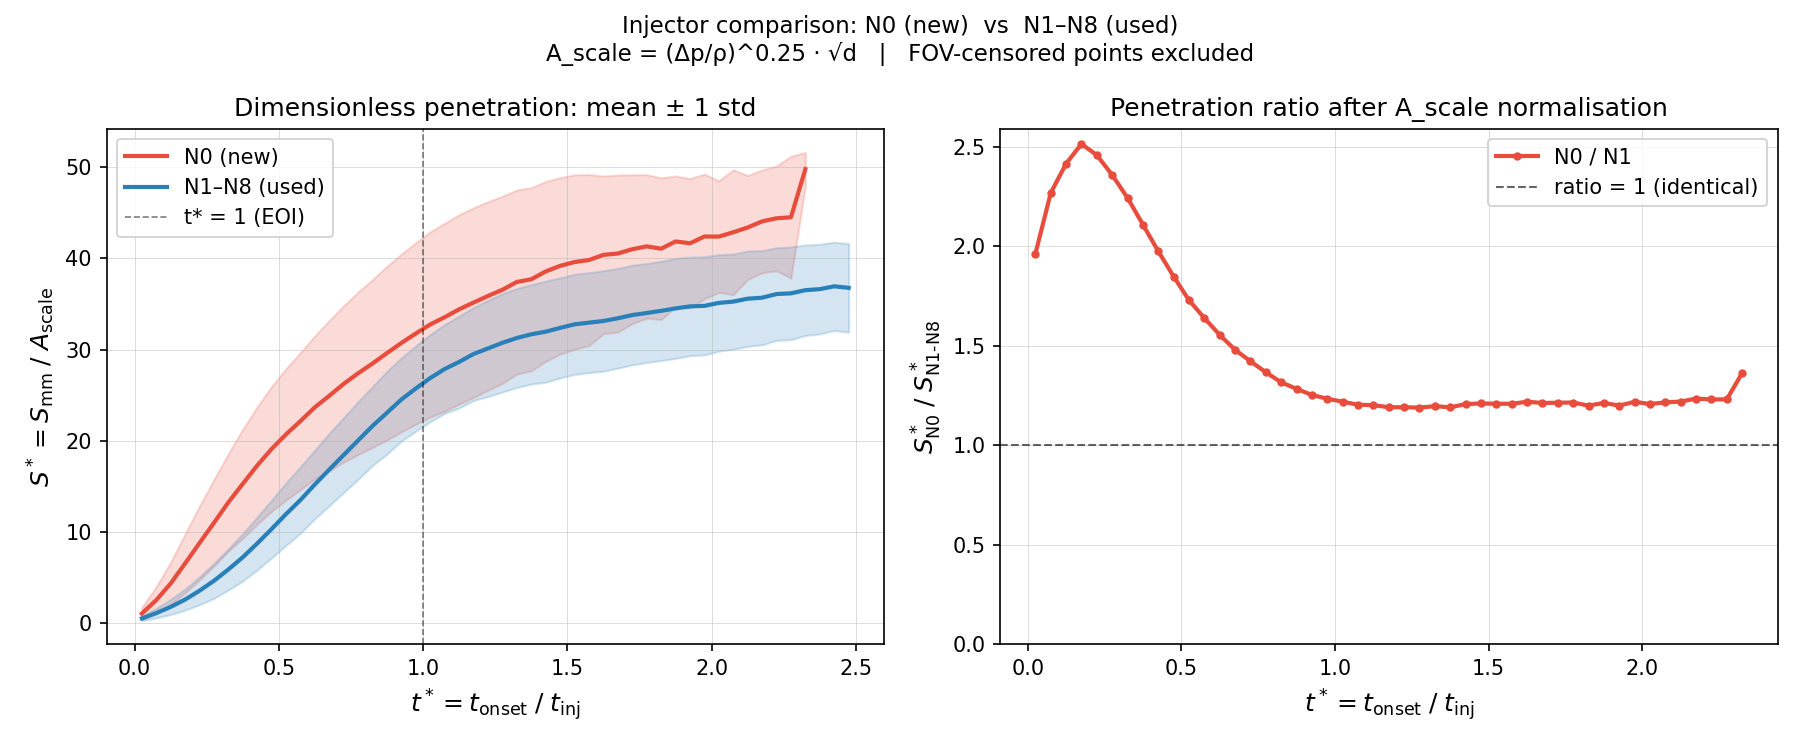
\includegraphics[width=\linewidth,height=5.0cm,keepaspectratio]{figs/injector_comparison.png}
\end{center}
\end{columns}
\end{frame}

% ──────────────────────────────────────────────────────────────
\begin{frame}{Family-Aware Head: Design}
\small
\begin{columns}[T]
\column{0.55\textwidth}
\textbf{\texttt{FamilyAwarePenetrationMLP}}
\begin{itemize}\setlength\itemsep{2pt}
  \item Shared trunk; drops the trailing \texttt{family\_id} channel.
  \item \texttt{mu\_heads}: per-family final heads (one $\mu$-output each).
  \item \texttt{log\_var\_head}: single shared variance head.
  \item Output $[\mu, \log\sigma^2]$ — drop-in for \texttt{PenetrationMLP}.
\end{itemize}

\vspace{0.3em}
\textbf{Routing}
\begin{itemize}\setlength\itemsep{2pt}
  \item Per-sample \texttt{family\_id} selects the head; trained families tracked
        via \texttt{trained\_families} buffer.
  \item Eval-time fallback: untrained families redirect to
        \texttt{fallback\_family\_id=1}.
\end{itemize}

\column{0.43\textwidth}
\begin{center}
\renewcommand{\arraystretch}{1.10}
\footnotesize
\begin{tabular}{@{}L{1.9cm}L{3.2cm}@{}}
\toprule
\textbf{Family} & \textbf{Members} \\
\midrule
0 (original) & Nozzle0 \\
1 (modified) & Nozzle1--8 \\
\bottomrule
\end{tabular}
\end{center}

\vspace{0.3em}
\footnotesize
Single head: one $\mu$-decoder on both families. Family head: two $\mu$-decoders
on a shared trunk; the variance head stays shared.
\end{columns}
\end{frame}

% ──────────────────────────────────────────────────────────────
\begin{frame}{Aggregate RMSE (mm, MLP\_series): Four Sweeps}
\small
\begin{center}
\renewcommand{\arraystretch}{1.22}
\setlength{\tabcolsep}{6pt}
\begin{tabular}{@{}lrrr@{}}
\toprule
\textbf{Run label} & \textbf{n folds} & \textbf{mean RMSE [mm]} & \textbf{std RMSE [mm]} \\
\midrule
\texttt{A\_single\_baseline}      & 5 & 11.44 & 10.76 \\
\texttt{B\_modified\_only}        & 5 & 12.71 & 13.58 \\
\rowcolor{winrow}
\texttt{C\_family\_head\_5fold}    & 5 & \textbf{7.35} & 2.45 \\
\rowcolor{winrow}
\texttt{C\_family\_head\_modified} & 5 & \textbf{6.56} & \textbf{0.90} \\
\bottomrule
\end{tabular}
\end{center}

\vspace{0.5em}
\begin{block}{Reading the table}
\begin{itemize}\setlength\itemsep{2pt}
  \item C vs A on \texttt{lono\_5fold}: $\Delta$ mean RMSE = \good{$-4.09$~mm}
        (11.44 $\to$ 7.35).
  \item C on \texttt{lono\_modified\_only}: \good{6.56~mm} mean RMSE,
        std collapsed by an order of magnitude (13.58 $\to$ 0.90).
  \item B alone (data filter without architectural change) is \emph{worse} than A:
        narrowing the training set hurts when the held-out fold is the
        second modified family.
\end{itemize}
\end{block}
\end{frame}

% ──────────────────────────────────────────────────────────────
\begin{frame}{Per-Fold RMSE: Where the Win Comes From}
\footnotesize
\begin{center}
\renewcommand{\arraystretch}{1.10}
\setlength{\tabcolsep}{4pt}
\begin{tabular}{@{}lrrrrr@{}}
\toprule
\textbf{Held-out nozzle} & \textbf{A\_single} & \textbf{B\_modified} & \textbf{C\_5fold} & \textbf{C\_modified} & \textbf{$\Delta$ (C vs A)} \\
\midrule
\rowcolor{warnrow}
Nozzle0 (original)       & \warn{30.58} & --            & \good{11.57}  & --            & \good{$-19.01$} \\
Nozzle1 (modified)       & 5.89         & 5.89          & 6.20          & 6.20          & $+0.31$ \\
Nozzle2 (modified)       & 8.37         & 8.37          & 7.36          & 7.36          & $-1.01$ \\
Nozzle4 (modified)       & 6.95         & 6.95          & 6.17          & 6.17          & $-0.78$ \\
Nozzle5 (modified)       & 5.41         & 5.41          & 5.46          & 5.46          & $+0.05$ \\
\rowcolor{warnrow}
Nozzle6 (modified)       & --           & \warn{36.91}  & --            & \good{7.61}   & \good{$-29.30$} \\
\midrule
\textbf{mean (own protocol)} & \textbf{11.44} & \textbf{12.71} & \textbf{7.35} & \textbf{6.56} & --- \\
\bottomrule
\end{tabular}
\end{center}

\vspace{0.4em}
\begin{itemize}\setlength\itemsep{2pt}
  \item Two folds carry the entire effect: Nozzle0 in \texttt{lono\_5fold}
        ($30.58 \to 11.57$) and Nozzle6 in \texttt{lono\_modified\_only}
        ($36.91 \to 7.61$).
  \item Four ``in-family'' modified folds (N1, N2, N4, N5) move by $\leq 1$~mm
        in either direction — well inside expected seed noise (Tier-1B).
  \item The family head does not hurt the easy folds; the win is paid for entirely
        by repairing the OOD-family folds.
\end{itemize}
\end{frame}

% ──────────────────────────────────────────────────────────────
\begin{frame}{Why B (Data Filter Alone) Underperforms}
\small
\begin{columns}[T]
\column{0.58\textwidth}
B keeps the production single-head architecture but trains only on the modified
family. On \texttt{lono\_modified\_only}, the held-out fold \emph{is itself} a
modified family member, so naively this should be a clean in-distribution
generalisation test.

\vspace{0.4em}
\textbf{The Nozzle6 catastrophe:}
\begin{itemize}\setlength\itemsep{2pt}
  \item B trains on modified $\setminus$ \{Nozzle6\}.
  \item Without Nozzle0 in the training set, the trunk has no exposure to the
        first-generation geometry; without family routing, the single $\mu$-decoder
        has no mechanism to specialise on the remaining modified subset either.
  \item Result: RMSE 36.91~mm on Nozzle6 — \emph{worse} than A's Nozzle0 collapse,
        despite N6 being in-design-family.
\end{itemize}

\column{0.40\textwidth}
\textbf{What this tells us}
\begin{itemize}\setlength\itemsep{3pt}
  \item Narrowing the training set is not a free lunch: it removes the implicit
        regularisation contributed by the other family.
  \item The relevant variable is \emph{routing capacity}, not
        \emph{training-set purity}.
  \item C\_modified, which keeps the same narrowed training set but adds the
        family head, drops Nozzle6 to 7.61~mm — a $-29.3$~mm gain attributable to
        the architecture change alone.
\end{itemize}
\end{columns}

\vspace{0.4em}
\footnotesize
\textbf{Takeaway:} A vs B vs C\_modified is a clean three-way ablation isolating
\emph{architecture} from \emph{training-set composition}. Architecture wins.
\end{frame}

% ──────────────────────────────────────────────────────────────
\begin{frame}{Why C Wins on Nozzle0 (5-fold)}
\small
On \texttt{lono\_5fold}, Nozzle0 is the only first-generation injector geometry and
the only member of family~0. When N0 is held out, family~0's $\mu$-head sees
\emph{zero training samples}.

\vspace{0.4em}
\begin{block}{Eval-time routing for held-out N0}
The model uses the fallback mechanism: \texttt{family\_id=0} samples at eval time
are redirected to the family-1 ($\mu$-head) via \texttt{fallback\_family\_id=1}.
The shared trunk still encodes general spray dynamics; the family-1 head supplies
the $\mu$-mapping it learned from the modified family.
\end{block}

\begin{block}{Why this beats A's monolithic decoder}
\begin{itemize}\setlength\itemsep{2pt}
  \item A trained on a mixture (1{,}038 N0 vs $\sim$600 modified). With N0 held out,
        the decoder is pulled toward family-0 geometry by samples that no longer apply.
  \item C's family-1 head was trained \emph{only} on modified samples, producing a
        cleaner extrapolation surface for the unseen family-0 geometry.
  \item Result: N0 RMSE collapses from $30.58 \to 11.57$~mm. Still above the in-family
        $\sim$5--7~mm band, but no longer catastrophic --- the family head makes
        extrapolation \emph{less wrong}, not correct.
\end{itemize}
\end{block}
\end{frame}

% ──────────────────────────────────────────────────────────────
\begin{frame}{Caveats Before Declaring Victory}
\small
\begin{block}{Seed variance not yet quantified}
The Tier-1B \texttt{run\_seed\_variance.py} sweep (5 seeds $\times$ Nozzle2 LONO)
has not been replayed for the family-head architecture. Until $\sigma_{\text{seed}}$
is measured, the in-family deltas ($\leq 1$~mm on N1, N2, N4, N5) cannot be
interpreted as real improvements. The N0 and N6 deltas (19--29~mm) are too large
to be seed noise.
\end{block}

\begin{block}{Nozzle0 is still not a converged fold}
C\_5fold's N0 RMSE of 11.57~mm sits 2--3$\times$ above the in-family band.
Family-aware routing has moved N0 from ``catastrophic'' to ``noticeably degraded'',
not to ``in-family''. Reporting C as a fix for OOD geometry would be overclaiming.
The honest framing: C reduces the OOD penalty without eliminating it.
\end{block}

\begin{block}{Fallback policy is a hyperparameter}
The choice \texttt{fallback\_family\_id=1} is hard-coded. Alternative policies
(softmax over trained heads, learned routing) were not evaluated in this sweep.
\end{block}
\end{frame}

% ──────────────────────────────────────────────────────────────
\begin{frame}{From LONO Teacher to Deployed Student}
\small
The sweep above scores the \emph{Stage-2 teacher}. Production deploys the
\emph{Stage-3 distillation student}, which was hard-coded single-head, so the
proven family routing was \warn{discarded after distillation}. Three changes ship
it into the deployed model:
\begin{itemize}\setlength\itemsep{2pt}
  \item Stage-3 student is now \texttt{FamilyAwarePenetrationMLP} ($[\mu,\log\sigma^2]$),
        warm-started verbatim from the family-head teacher.
  \item Onset auxiliary head removed (onset alignment now $\pm$ a few $\mu$s;
        inference already dropped that channel).
  \item Whole chain on \texttt{a\_dp050\_plus\_pressures} (7 features $+$ \texttt{family\_id}).
\end{itemize}

\begin{block}{Divergence $\to$ frozen-trunk fix}
Naively refining the warm-started student \warn{diverges}: majority-family
(N1--8) raw-NLL gradients drift the shared trunk, the minority family-0 head
cannot track it, and the KD $\sigma$-term explodes
(val KD $0.9\!\to\!51$, best $=$ epoch~1). \good{Freezing the trunk}
(334.7\,k params fixed, 49.9\,k head params trained) restores stable refinement
(val KD $\approx 0.2$, converges $\sim$epoch~78).
\end{block}
\end{frame}

% ──────────────────────────────────────────────────────────────
\begin{frame}{Deployed Student: Corrected Evaluation}
\footnotesize
\textbf{Eval pitfall:} the \texttt{clean} series still contains right-censored
FOV-tail points; as headline metric it inflates RMSE and fakes an under-prediction
bias. Primary metric switched to the \emph{uncensored} point table
(\texttt{cdf\_uncensored}, 543\,k points).

\smallskip
\begin{center}
\renewcommand{\arraystretch}{1.1}
\setlength{\tabcolsep}{5pt}
\begin{tabular}{@{}lrrrr@{}}
\toprule
\textbf{Stage-3 student} & \textbf{clean RMSE} & \textbf{unc.\ RMSE} & \textbf{unc.\ bias} & \textbf{unc.\ cov$_{1\sigma}$} \\
\midrule
unfrozen ($\lambda_{\rm a}{=}0$)         & 8.91 & \warn{9.80} & \warn{$-3.11$} & \warn{0.47} \\
\rowcolor{winrow}
frozen ($\lambda_{\rm a}{=}0$) [deploy]  & 8.54 & \good{5.01} & \good{$+0.67$} & \good{0.85} \\
\bottomrule
\end{tabular}
\end{center}

\begin{columns}[T]
\column{0.55\textwidth}
\textbf{Freeze is a $\sim$2$\times$ win, not marginal.} The censored \texttt{clean}
metric masked it ($-0.37$~mm); uncensored, the gap is $9.80\!\to\!5.01$ with
calibration restored ($0.47\!\to\!0.85$). The earlier ``N0 under-predicts
$\sim$8~mm'' was a censoring artifact (uncensored bias $\approx 0$).

\column{0.43\textwidth}
\textbf{Open problem: extrapolation.}\\[2pt]
\begin{tabular}{@{}lrr@{}}
\toprule
region & RMSE & bias \\
\midrule
in-window     & \good{3.7}  & $+1.2$ \\
extrapolated  & \warn{11.3} & \warn{$+7.4$} \\
\bottomrule
\end{tabular}\\[2pt]
In-window is calibrated; error is \emph{over-prediction} beyond the horizon.
\end{columns}
\end{frame}

% ──────────────────────────────────────────────────────────────
\begin{frame}{Stage-3 Partial Unfreeze Check}
\scriptsize
\textbf{Setup:} family-head baseline freezes the shared trunk; new run unfreezes
only the last trunk block with trunk LR $3{\times}10^{-5}$ and head LR $3{\times}10^{-3}$.

\begin{center}
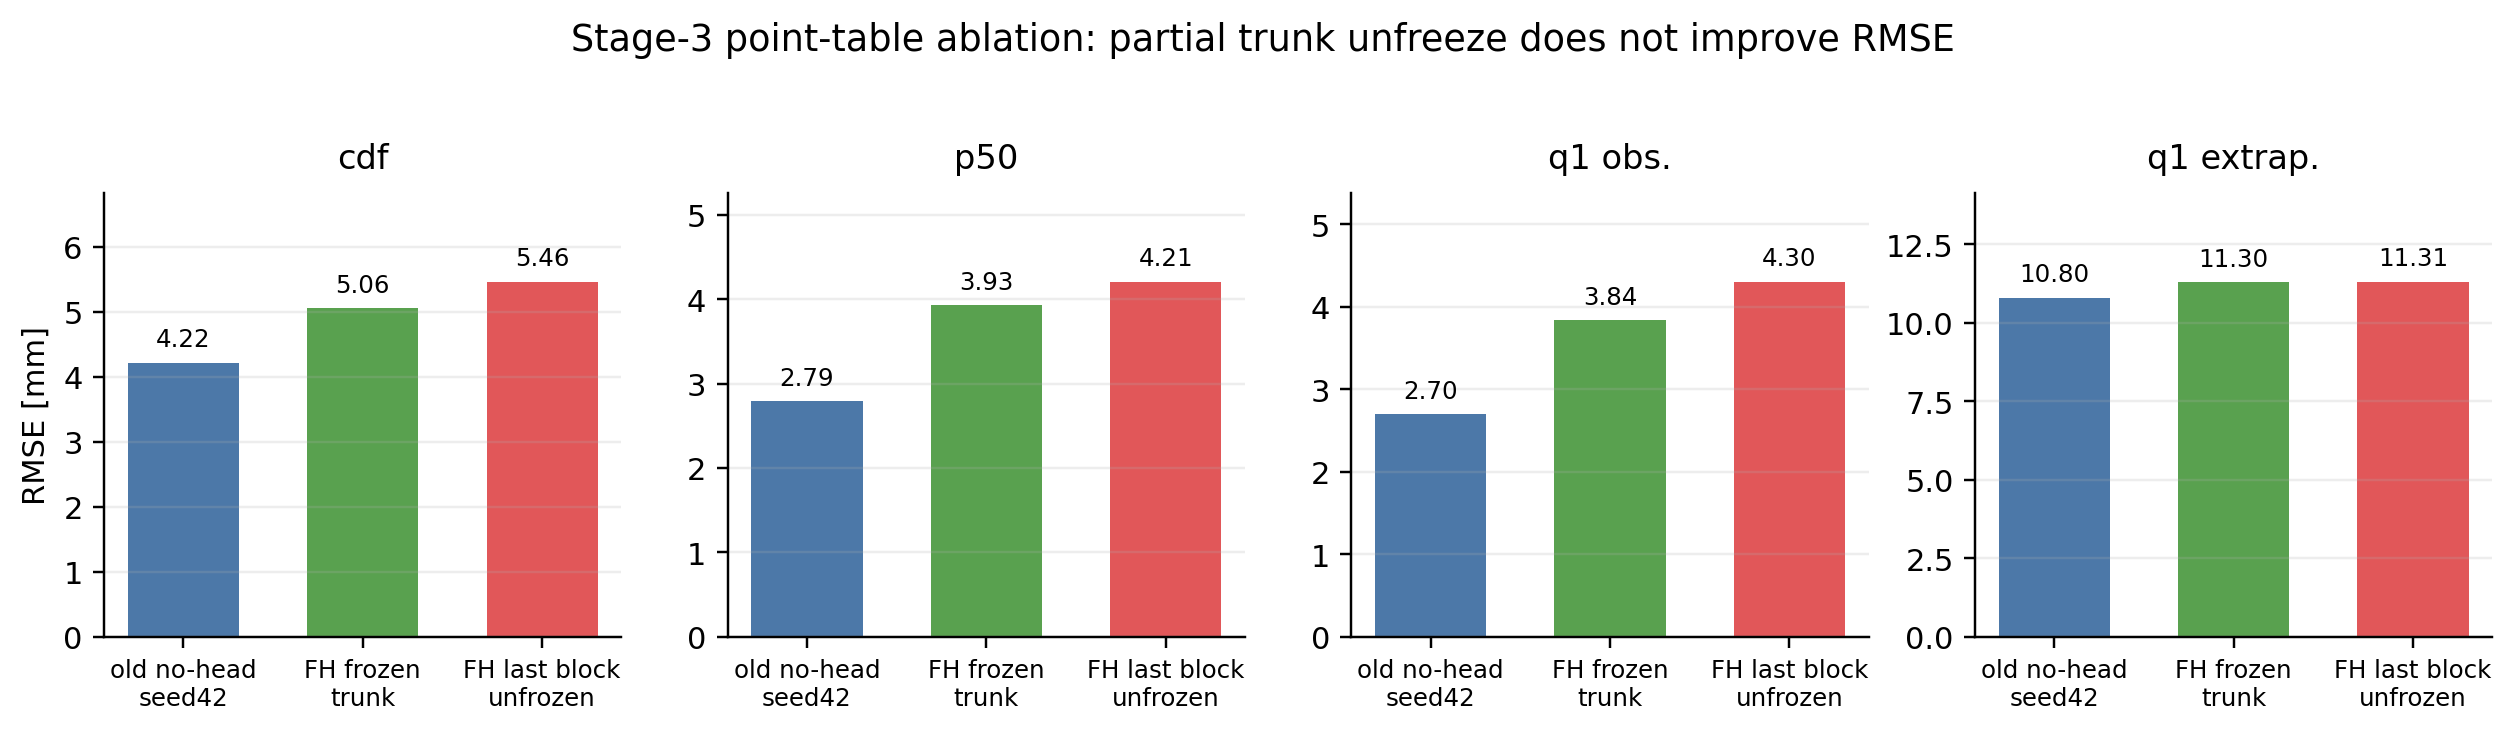
\includegraphics[width=0.84\textwidth]{figs/stage3_partial_unfreeze_rmse.png}
\end{center}
\vspace{-1.0em}

\begin{center}
\renewcommand{\arraystretch}{1.02}
\setlength{\tabcolsep}{4pt}
\begin{tabular}{@{}lrrrr@{}}
\toprule
\textbf{Stage-3 point-table run} & \textbf{cdf RMSE} & \textbf{p50 RMSE} & \textbf{cdf ECE} & \textbf{cdf CRPS} \\
\midrule
old no-head seed42              & \good{4.22} & \good{2.79} & 0.0778 & \good{2.30} \\
family-head, frozen trunk       & 5.06 & 3.93 & 0.0708 & 2.80 \\
family-head, last block unfrozen & \warn{5.46} & \warn{4.21} & \good{0.0513} & 2.72 \\
\bottomrule
\end{tabular}
\end{center}

\vspace{-0.1em}
\textbf{Takeaway:} partial unfreezing improves scalar calibration but worsens
point accuracy on every headline eval set; keep the frozen trunk.
\end{frame}

% ──────────────────────────────────────────────────────────────
\begin{frame}{Conclusion}
\footnotesize
\begin{enumerate}\setlength\itemsep{2pt}
  \item C (family-aware head) is the decisive winner on both LONO protocols:
        \texttt{lono\_5fold} $11.44\!\to\!7.35$~mm ($-4.09$); \texttt{lono\_modified\_only}
        $6.56$~mm with std $13.58\!\to\!0.90$.
  \item The win is concentrated on two OOD-family folds --- Nozzle0
        ($30.58\!\to\!11.57$) and Nozzle6 ($36.91\!\to\!7.61$); in-family folds move
        $\leq 1$~mm.
  \item A vs B vs C\_modified isolates \emph{architecture} from \emph{training-set
        composition}: B (filter alone, 12.71) loses to A (11.44); C\_modified
        (architecture, 6.56) wins. Routing capacity is the decisive variable.
  \item \textbf{Deployed model:} the Stage-3 student is now family-aware with a
        \emph{frozen trunk} (onset head dropped). On the uncensored point-table metric
        it reaches \good{$5.0$~mm} RMSE / $+0.7$~mm bias / $0.85$ coverage, vs
        $9.8$~mm unfrozen; remaining error is extrapolation over-prediction.
  \item New partial-unfreeze check: unfreezing only the last trunk block at
        LR $3{\times}10^{-5}$ does \warn{not} improve the Stage-3 student
        (cdf RMSE $5.06\!\to\!5.46$, p50 RMSE $3.93\!\to\!4.21$). Next
        ablation should use residual family heads or adapters, not shared-trunk drift.
  \item Caveat: Tier-1B seed-variance still pending before claiming the in-family
        $\leq 1$~mm deltas are real.
\end{enumerate}

\vspace{0.2em}
\scriptsize
\textbf{Artifacts:}
\texttt{family\_head\_sweep\_20260528\_212646/} (LONO);
\texttt{distill\_cdf\_family\_head\_v3\_FROZEN\_anchor\_off\_20260529\_213346/} (deployed);
\texttt{stage3\_partial\_unfreeze\_ablation.csv} (partial-unfreeze);
\texttt{MLP/eval/inference\_rmse\_on\_point\_tables.py} (uncensored metric).
\end{frame}

\end{document}
